\section{t-Closeness}

\begin{frame}{t-Closeness}
	t-closeness stellt ein Maß für minimalen Wissensgewinn, der durch Betrachtung eines q*-Blocks im Vergleich zur gesamten Distribution entsteht, dar \cite{kltHauf}.

	\begin{block}{Definition t-closeness}
		Eine \textbf{Äquivalenzklasse} (q*-Block) hat die Eigenschaft \textbf{t-closeness}, wenn die (semantische) Distanz zwischen der Verteilung der Werte eines sensiblen Attributes innerhalb der Äquivalenzklasse und der Verteilung der Werte des sensiblen Attributes innerhalb der Tabelle nicht größer als \(t\) ist. 

		Eine \textbf{Tabelle} hat die Eigenschaft \textbf{t-closeness}, wenn diese Eigenschaft für alle Äquivalenzklassen erfüllt ist.	
	\end{block}

	\textbf{Problem}: Wie bestimmt man die (semantische) Distanz?
\end{frame}

\subsection{Earth Movers Distanz (EMD)}

\begin{frame}{Earth Movers Distanz (EMD)}
	Die Earth Movers Distanz (EMD) basiert auf der minimalen Arbeit, die zu verrichten ist, um eine Verteilung in eine andere zu überführen.
	\begin{block}{Definition von EMD \cite{Li2007t-closseness}}
		Gegeben sei $P=(p_1,...,p_m)$, $Q=(q_1,...,q_m)$, $d_{ij}$ ist die Grunddistanz zwischen $p_i$ und $q_j$. $f_{ij}$ ist die minimale Masse, die transportiert werden muss, um $p_i$ in $q_j$ zu verwandeln. EMD ist dann die gesamte Arbeit, die verrichtet werden muss $D[P,Q] = \sum_{i=1}^m \sum_{j=1}^m d_{ij} f_{ij}$\\
		unter den folgenden Bedingungen
		\begin{enumerate}[i)]
			\item $f_{ij}\ge 0$ | $1\le i \le m, 1\le j \le m$		
			\item $p_i - \sum_{j=1}^{m}f_{ij} +\sum_{j=1}^{m}f_{ji} = q_i$ | $1 \le i \le m$
			\item $\sum_{i=1}^{m}\sum_{j=1}^{m} f_{ij} = \sum_{i=1}^{m} p_i = \sum_{i=1}^{m} q_i$ 
		\end{enumerate}
	\end{block}
\end{frame}

\begin{frame}{Earth Movers Distanz (EMD)}
	Aus den drei Bedingungen folgen die zwei Fakten \cite{Li2007t-closseness}:\\
	\ \\
	\textbf{Fakt 1:} If $\forall i,j | 0 \le d_{ij} \le 1$ then $0 \le D[P,Q]  \le 1$. 
	Das bedeutet, dass wenn die Grunddistanz normalisiert ist, auch die EMD normalisiert ist. \textbf{Somit kann ein einheitliches Maß für t bestimmt werden.}\\
	\ \\
	\textbf{Fakt 2:} Gegeben sind zwei Äquivalenzklassen $E_1$ und $E_2$.
	$P_1$ ist die Verteilung eines sensiblen Attributes aus $E_1$.
	$P_2$ ist die Verteilung eines sensiblen Attributes aus $E_2$.
	$P$ ist die Verteilung eines sensiblen Attributes aus $E_1 \cup E_2$. Dann gilt die folgende Ungleichung: \\
	$D[P,Q] \le \frac{|E_1|}{|E_1|+|E_2|}D[P_1,Q] + \frac{|E_2|}{|E_1|+|E_2|}D[P_2,Q]$\\
	$\Rightarrow D[P,Q] \le max(D[P_1,Q], D[P_2,Q])$ 
\end{frame}

\begin{frame}{Earth Movers Distanz (EMD)}
	\textbf{Fakt 2:} $D[P,Q] \le max(D[P_1,Q], D[P_2,Q])$ 
	Dies bedeutet, dass die maximale Distanz zwischen einer Äquivalenzklasse und der Tabelle beim Zusammenführen zweier Äquivalenzklassen nicht steigt. \textbf{Somit bleibt die t-closeness-Eigenschaft beim Zusammenführen erhalten.} \\ 
	\ \\
	\textbf{Generalisation Property:} Sei $T$ eine Tabelle, $A$ und $B$ sind Generalisierungen von $T$, wobei $A$ mehr generalisiert ist als $B$. Wenn $B$ die Eigenschaft t-closeness hat, dann hat auch $A$ die Eigenschaft t-closeness.\\
	\ \\
	\textit{Beweis:} Die Äquivalenzklassen aus $A$ bestehen aus der Vereinigung mehrerer Äquivalenzklassen aus $B$. Nach Fakt 2 kann somit die maximale Distanz nicht größer werden. Somit hat auch $A$ die Eigenschaft t-closeness.  
\end{frame}

\begin{frame} {EMD Beispiel}
	
	\begin{columns}[T]
		\begin{column}{0.5\textwidth}
			\begin{table}[]
				\centering
				\label{tclossenessExample}
				\begin{tabular}{|l|l|l|}
					\hline
					\textbf{PLZ}   & \textbf{Alter}    & \textbf{Einkommen} \\\hline
					4767* & $\le 40$ & 3K \\
					4767* & $\le 40$ & 4K \\
					4767* & $\le 40$ & 5K \\\hline
					4790* & $\ge 40$ & 6K \\
					4790* & $\ge 40$ & 8K \\
					4790* & $\ge 40$ & 11K \\\hline
					4760* & $\le 40$ & 7K \\
					4760* & $\le 40$ & 9K \\
					4760* & $\le 40$ & 10K \\\hline
				\end{tabular}
				\caption{Einkommenstabelle}
			\end{table}
		\end{column}
		
		\begin{column}{0.5\textwidth}
			$Q = \{3k, 4k, 5k, 6k, 7k, 8k, 9k, 10k, 11k\}$\\
			\ \\
			$P_1 = \{3k, 4k, 5k\}$ \\
			$P2 = (\{6k, 8k, 11k\})$ 
			$P3 = (\{7k, 9k, 10k\})$
			\ \\
			\ \\
			\tiny Beispiel aus \cite{Li2007t-closseness}
		\end{column}
	\end{columns}
\end{frame}
\subsection{EMD Formeln} 
\begin{frame}{EMD Formeln}
	\textbf{Nummerische Attribute:} \\
	Domäne: $\{v_i,...,v_m\}$, wobei gilt $i<j \Rightarrow v_i \le v_j$\\
	\ \\
	geordnete-Distanz($v_i,v_j$)= = $\frac{|i-j|}{m-1}$
\end{frame}
\begin{frame}{EMD Formeln}
	\begin{figure}
		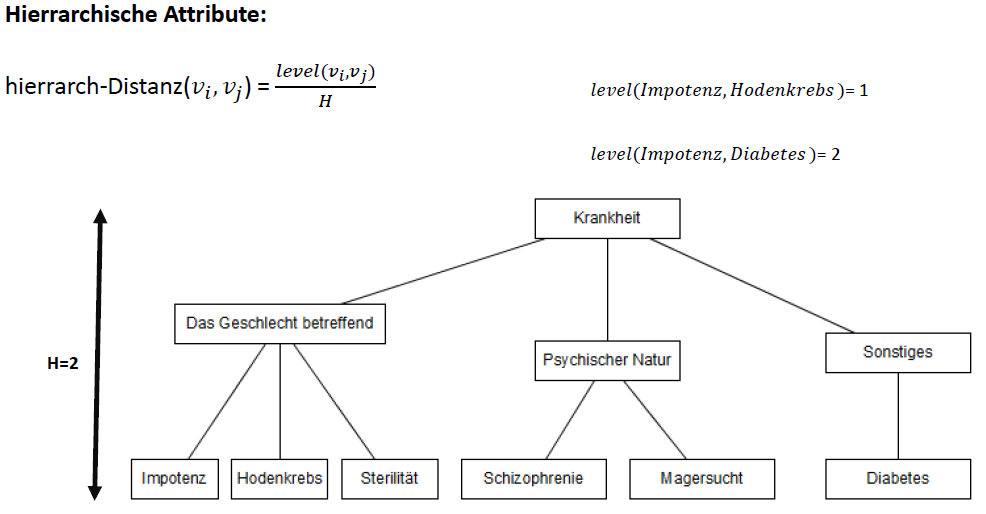
\includegraphics[scale=0.51]{pic/EMD_Formel.png}
	\end{figure}
\end{frame}
\subsection{EMD Beispiel}
\begin{frame}{EMD Beispiel}
	$Q = \{3k, 4k, 5k, 6k, 7k, 8k, 9k, 10k, 11k\}$\\
	$P_1 = \{3k, 4k, 5k\}$ \\
	Wahrscheinlichkeit $\frac{1}{9}$ für folgende Transition:
	$(5k\rightarrow 11k), (5k\rightarrow 10k), (5k \rightarrow 9k),
	(4k \rightarrow 8k), (4k\rightarrow 7k), (4k \rightarrow 6k), (3k\rightarrow 5k), (3k\rightarrow 4k), (3k \rightarrow 3k).$\\
	\ \\
	$\Rightarrow D[P_1,Q]= \frac{1}{9} \cdot \frac{6 + 5 + 4 + 4 + 3 + 2 + 2 + 1 + 0}{9-1} = 27/72 = 3/8 = 0.375$
\end{frame}
\begin{frame} {EMD Beispiel}
	
	\begin{columns}[T]
		\begin{column}{0.5\textwidth}
			\begin{table}[]
				\centering
				\label{tclossenessExample}
				\begin{tabular}{|l|l|l|}
					\hline
					\textbf{PLZ}   & \textbf{Alter}    & \textbf{Einkommen} \\\hline
					4767* & $\le 40$ & 3K \\
					4767* & $\le 40$ & 4K \\
					4767* & $\le 40$ & 5K \\\hline
					4790* & $\ge 40$ & 6K \\
					4790* & $\ge 40$ & 8K \\
					4790* & $\ge 40$ & 11K \\\hline
					4760* & $\le 40$ & 7K \\
					4760* & $\le 40$ & 9K \\
					4760* & $\le 40$ & 10K \\\hline
				\end{tabular}
				\caption{Einkommenstabelle}
			\end{table}
		\end{column}
		
		\begin{column}{0.5\textwidth}
			$D[P_1,Q]=\frac{27}{72} = 0,375$\\
			\ \\
			$D[P_2,Q]=\frac{12}{72} = 0,167$\\
			\ \\
			$D[P_3,Q]=\frac{17}{72} = 0,236,$\\
			\ \\
			$\Rightarrow t=0,375$\\
			\ \\
			Die Einkommenstabelle hat die Eigenschaft 0,375-closeness	
		\end{column}
	\end{columns}
\end{frame}
\begin{frame} {EMD Beispiel}
	
	\begin{columns}[T]
		\begin{column}{0.5\textwidth}
			\begin{table}[]
				\centering
				\label{tclossenessExample}
				\begin{tabular}{|l|l|l|}
					\hline
					\textbf{PLZ}   & \textbf{Alter}    & \textbf{Einkommen} \\\hline
					4767* & $\le 40$ & 3K \\
					4767* & $\le 40$ & 5K \\
					4767* & $\le 40$ & 9K \\\hline
					4790* & $\ge 40$ & 6K \\
					4790* & $\ge 40$ & 8K \\
					4790* & $\ge 40$ & 11K \\\hline
					4760* & $\le 40$ & 4K \\
					4760* & $\le 40$ & 7K \\
					4760* & $\le 40$ & 10K \\\hline
				\end{tabular}
				\caption{Einkommenstabelle}
			\end{table}
		\end{column}
		
		\begin{column}{0.5\textwidth}
			$D[P_1^{'},Q]=\frac{12}{72} = 0,167$\\
			\ \\
			$D[P_2,Q]=\frac{12}{72} = 0,167$\\
			\ \\
			$D[P_3^{'},Q]=\frac{6}{72} = 0,083,$\\
			\ \\
			$\Rightarrow t=0,167$\\
			\ \\
			Die Einkommenstabelle hat die Eigenschaft 0,167-closeness	
		\end{column}
	\end{columns}

\end{frame}

\section{Fazit}

\begin{frame}{Fazit}
	\begin{itemize}
		\item k-Anonymität
		\begin{itemize}
			\item mindestens $k$ Tupel mit identischem Quasi-Identifikator
		\end{itemize}

		\item l-Diversität
		\begin{itemize}
			\item mindestens $l$ verschiedene sensible Werte in jeder Äquivalenzklasse
		\end{itemize}

		\item t-Closeness
		\begin{itemize}
			\item Distanz zwischen Verteilung der sensiblen Attribute einer Äquivalenzklasse und der Gesamtverteilung unterscheidet sich maximal um einen Schwellwert \(t\)
		\end{itemize}

		\pause

		\item Ausblick
		\begin{itemize}
			\item gewichtete Attribute
			\item Schwellwerte für maximale Anzahl an unterdrückten Tupeln
			\item mehrere sensible Attribute
			\item ...
		\end{itemize}
	\end{itemize}
	%	Zusätzlich (und hier nicht abgedeckt): gewichtete Attribute, Schwellwerte für maximale Anzahl an unterdrückten Tupeln, mehrere sensible Attribute, ...
\end{frame}